\chapter{引言}
\label{cha:intro}
本文提出CloudVision分布式机器视觉云平台,让机器视觉研究人员
可以高效,按需地执行大规模数据的机器视觉任务。本章\ref{sec:background}对论文涉及的
相关领域,包括机器视觉,大数据和云计算进行简单介绍,了解到CloudVision跟
三个领域的关系。
在本章\ref{sec:challenges}描述CloudVision解决的问题与创新点。
最后在本章\ref{sec:main_work}总结主要工作和论文结构。

\section{研究背景}
\label{sec:background}
近年来,机器视觉在各个领域得到广泛的应用,如自动驾驶小车,监控,医疗,交通,IoT,机器人等等。
机器视觉得以蓬勃发展,与大数据和云计算技术息息相关。
新的应用依赖海量数据输入,使用机器视觉算法,同时要求其计算能力随数据的增长而提高。
CloudVision平台使用大数据和云计算领先的方法,提供一个稳定的,针对海量数据的机器视觉执行平台。

机器视觉专门研究怎么用计算机理解可视化的数据,比如使用
从摄影机的图像或者视频,用可视化的数据识别人脸,车或者物体。
最开始机器视觉的研究因为存储和计算能力有限,专注于
小的数据集,比如LeCunn在1989年的神经网络的研究使用了MNIST数据集,
他计算器使用了一个SUN-4/260。\cite{lecun1989backpropagation}
SUN-4/260的CPU是16.67Mhz和最多支持128MB RAM,如果用现在最佳的
机器视觉方法执行在当时的机器,需要执行几年的时间。机器视觉的
一个重要部分是训练数据的大小,如果用更多的数据一般能达到
更好的效果。现在的机器视觉的研究都使用更大的数据集,
另外新的算法对计算能力的要求也增加了,一般要求执行
在大量的CPU和GPU集群。\cite{googlenet2015,baidup2015deepgpu}
在章\ref{subsec:cv_background}详细介绍机器视觉的现状。

大数据领域专门研究大数据集如何保存和处理,用处理的数据提供价值。
世界的数据不停的在增长,比如城市里的监控数据,互联网的视频网站。传统
的单处理系统无法保存和处理海量的数据。因此大数据一般分布到集群,然后整个集群
并行处理数据。为了解决机器视觉的海量数据存储和处理问题,可以使用
大数据领域方法。在章\ref{subsec:bigdata_background}详细介绍大数据领域的现状。

云计算是一种模式,通过互联网按需提供计算和存储资源。多个用户可以随时随地使用
共享计算资源池(比如服务器,存储,网络,应用,服务)。
为了使得机器视觉能够弹性的处理大数据,可以使用云计算提供灵活的计算基础设施。
在章\ref{subsec:cloud_background}详细介绍云计算的模型和现状。




\section{问题与挑战}
\label{sec:challenges}
大数据的技术虽然能改善机器视觉,但是同时也带来新的问题与挑战。
CloudVision想解决的挑战:
\begin{itemize}
  \item 扩展性 \\
        机器视觉最大挑战是扩展性。随着数据的不断增加,系统必须能够弹性地增加存储能力和计算能力,
        从而保证机器视觉算法的可执行性和高效性。与传统的在一台机器上运行机器视觉算法不同,
        将机器视觉运行在集群上,在多个计算节点上并行执行是非常重要的需求。
  \item 基础设施可用性 \\
        基础设施可用性的挑战来自规模和特性。很多大学和研究机构没有大型数据中心专门给研究使用。
        最先进的基于深度学习算法使用大量的CPU或者GPU集群\cite{googlenet2015, google2015rethinking, baidup2015deepgpu}。
        “百度深度学习研究院”用了一个定制的超计算机,里面有34个服务器,每台有两块6核Intel Xeon E5-2620,4个
        Nvidia Tesla K40m GPU,用低延迟的InfiniBand组成一个408个CPU核和136个GPU集群。“Baidu深度学习研究院”基于这个集群,
        通过增加数据训练机器学习的模型,达到了更先进的结果。\cite{baidup2015deepgpu}
        从中可以看出基础设施的重要性,像Baidu这类大型公司,一般拥有大的数据中心和基础设施设计的专家。
        但是大学或者研究机构一般比较缺乏对基础设施的建设。
  \item 并行化 \\
        通过并行化可以解决扩展性的挑战,但是设计并行化的程序也是一个挑战。设计和实现并行化的程序得考虑
        很多方面,包括数据转播,怎么分任务并行执行等等。
  \item 运维负担 \\
        部署,维护和管理需要一定的运维能力和投资。大的集群超过1000个服务器,需要自动化的运维。
        得有运维专家专门运维处理集群,了解具体的软件和基础设施。
  \item 易用性 \\
        目前的主流软件比如OpenCV都需要用户自己安装和部署,解决依赖关系问题等等。这个是一个耗费经历的工作。
        另外如果要在集群上配置OpenCV,其环境的安装和维护将更加复杂。
  \item 可重用性 \\
        机器视觉的研究员经常需在原有的算法做改进或者研究新的算法。他们需要对比新的算法跟目前主流算法的
        准确性,计算时间等等。目前经常需要重新实现原有的算法,浪费大家的时间,因此需要提高可重用性。
  \item 高性能 \\
        高性能挑战主要考虑计算时间和计算的瓶颈,比如集群里的数据传速,硬盘IO等等。
\end{itemize}

\section{相关工作}
\label{sec:related_work}

\subsection{VMX Object Detection/Recognition System}
Vision.ai公司的VMX产品是一个实时的物体检测和分类软件,可以通过Web界面或者RESTful API使用。
VMX提供的物体检测算法专注于速度和准确性,可以快速学习新的模型,将新的模型用来检测,分类,和
跟踪图像或视频里的物体。VMX简单化机器视觉应用在生活中的应用。

\subsection{CloudCV}
CloudCV提供大规模分布式的机器视觉云服务。
CloudCV通过Web界面或者API方式提供最先进的机器视觉算法。整个系统是开源的。\cite{cloudcv2015}

\begin{wrapfigure}{r}{0.50\textwidth}
  \centering
    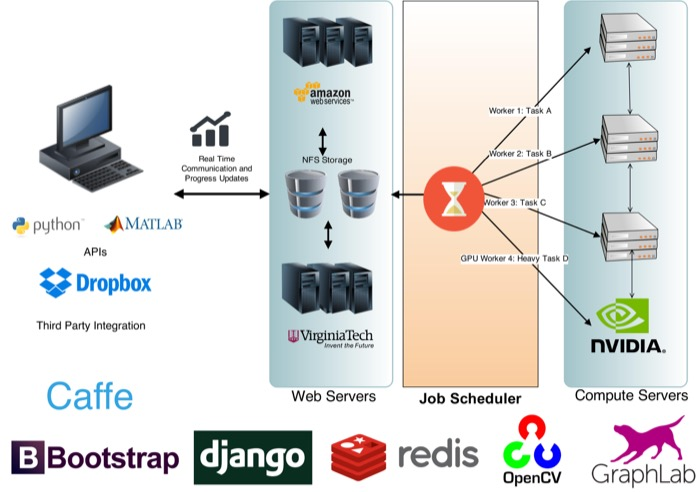
\includegraphics[width=0.49\textwidth]{cloudcv-architecture}
    \caption{CloudCV系统架构。\cite{cloudcv2015}}
  \label{fig:cloudcv-arch}
\end{wrapfigure}
在图\ref{fig:cloudcv-arch}可以看到CloudCV系统的架构。Web Servers基于Django的Web开发框架提供
一个HTTP API和界面。API暴露的接口有:图片分类,DeCAF特征抽取,图像人物识别,
Image Stitcing。数据保存到一个NFS(Linux Network File System)服务器。
在任务调度方面,CloudCV使用Python的Celery框架,为每个节点分配特定的任务。
它们通过不同的队列将任务调度到不同的节点组。按任务类型分队列,这样可以将需要GPU的任务调度
到有GPU的节点。所有计算节点从信息队列中收到需要执行的任务。计算节点使用AWS,Azure和Virginia内部
云平台提供基础设施资源。机器视觉任务主要基于Caffe和OpenCV实现。

\subsection{相关工作结论}
VMX和CloudCV都使得机器视觉的执行更加简单。VMX是一个专有软件,CloudCV是一个开源软件。
两个系统都缺乏一个研究员的场景,允许研究员自己定制算法并大规模执行。CloudCV和VMX主要针对
用一些他们包装好的算法但是没有提供一个可以执行自己的机器视觉应用的平台。另外也没有提供
大数据存储的能力,现实生活中的数据集越来越大,需要一个分布式存储保存。CloudCV用到的NFS无法
扩展到大规模使用。

\section{本文主要工作}
\label{sec:main_work}

本论文工作主要是基于大数据和云计算模型,实现大规模分布式机器视觉执行平台CloudVision。
本节将简单介绍论文三个工作重点:
\begin{itemize}
  \item 大数据,云计算和机器视觉的混合研究

        为了提供一个更好符合现在的研究员的平台,我首先
        研究了机器视觉主流方法和实现。目前机器视觉研究面对数据大小和处理需求的增长。其他的研究领域
        解决类似的问题,所以为了不做重复的工作,我也研究和调研大数据和
        云计算的领域。

  \item CloudVision架构设计与实现

        基于大数据和云计算领先研究,设计CloudVision可扩展的架构。本文章描述
        CloudVision架构的细节和系统的实验方式。

  \item CloudVision平台建设及实验验证

        为了提供一个开发和实验环境,我建立了清华软件学院的信息系统与工程研究所的私有云。
        实验主要证明架构的选择和扩展性。

\end{itemize}


